\subsubsection{Machine Learning}
\index{Jaeger, Herbert}
\paragraph{Research Team}
Herbert Jaeger (Professor), Mingjie Zhao (Postdoctoral Fellow), Mantas Lukosevicius (PhD student)\\


Herbert Jaeger and his team develops Machine Learning methods for
the automated construction of prediction models from empirical
time series data.  Target applications (and collaborations) are in
the fields of neurobiology, human music understanding, handwriting
recognition, control engineering and telecommunication. Two main
methods investigated in Herbert Jaeger's group are recurrent
neural networks of the ``Echo State Network'' (ESN) type and
observable operator models (OOMs). ESNs are interesting not only
because they yield highly efficient learning algorithms but also
because they offer a biologically plausible model of learning in
natural brains. OOMs generalize hidden Markov models, a standard
tool in speech and text recognition, yielding more expressive
models in a fraction of the learning time required for hidden
Markov models. Both ESNs and OOMs have been originally found by
Herbert Jaeger and have been investigated in his group over the
last few years.



\paragraph{Highlights}

An important application of machine learning methods for time series
data is speech recognition. Almost all current methods in this field
rely on ``hidden Markov models'' as the basic machine learning
technique. Although recurrent neural networks (RNNs) would be more
plausible from a bionics perspective -- after all, our brains are RNNs
--, and although it is known that artificial RNNs can, in principle,
yield optimal speech signal decoders, these models have not in
practice been used due to the extreme computational cost and the
danger of instability of previously known training methods for RNNs.
RNNs of the Echo State Network type are computationally cheap to train
and intrinsically stable. Thus, one research direction in Jaeger's
group is to tailor ESNs to speech processing tasks.

A widely used benchmark task in this field is the ``Japanese Vowels''
problem\footnote{Data donated by Mineichi Kudo, Jun Toyama, and Masaru
  Shimbo; obtainable at \url{http://kdd.ics.uci.edu}}. The training
data consist of pre-processed vocal recordings from 9 Japanese
speakers, with 30 recordings per speaker. The task is to train from
these data a classificator that can recognize the speaker in test
recordings. Figure \ref{fig:JaegerFig1} shows some recordings from the
training set. The task is difficult because of high intra-speaker
 and low inter-speaker  variability. The best known classification
 methods achieve a test error rate of slightly less than 2 \%. Using
 ESN-based models with an unconventional architecture (combining the
 classification ``votes'' of 1,000 tiny ESNs with a particular neuron
 model which is more biologically plausible than standard artificial
 neuron models), Jaeger et al.\ achieved a \emph{zero} test error
 \cite{Jaegeretal2}.

\begin{figure}[ht]
  \begin{center}
   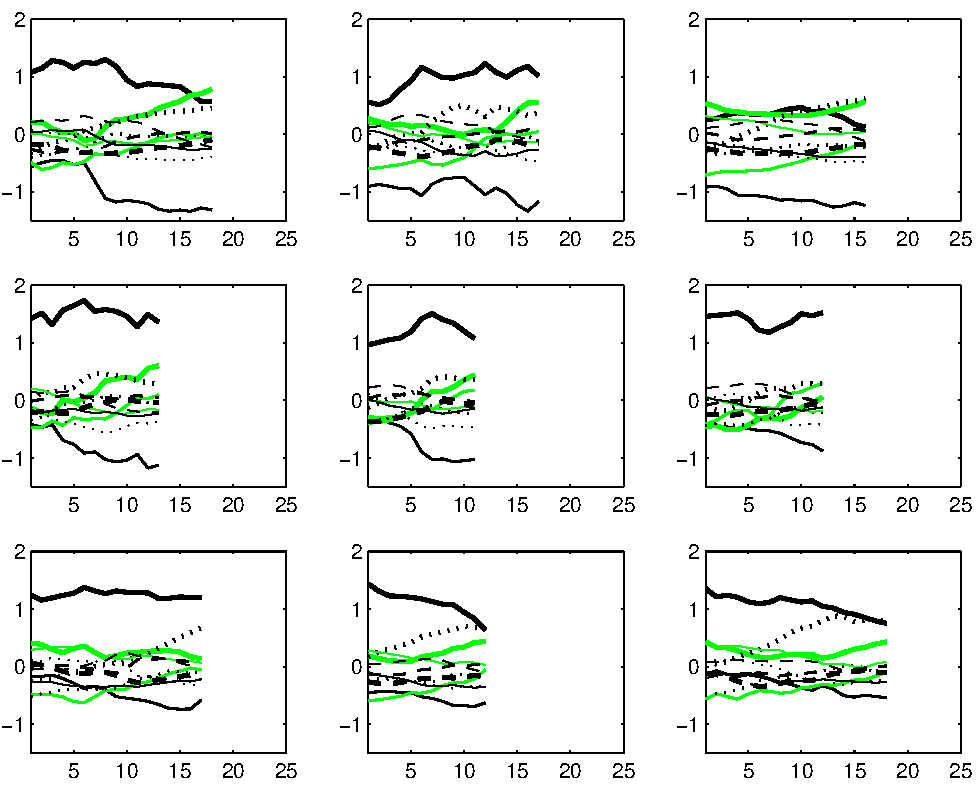
\includegraphics[width=\hsize]{JaegerFig1_2006.pdf}
    \caption{Some samples from the ``Japanese Vowels'' benchmark dataset. Each
    row shows three recordings from one speaker.}\label{fig:JaegerFig1}
   \end{center}
\end{figure}

Another important application of machine learning methods for time
series data is the recognition of handwritten texts. This task occurs,
for instance, in automated check reading systems or automated mail or
parcel sorting facilities. The text that is to be recognized is read
from left to right with a video reading head, yielding a video
sequence much like the visual input used by humans who read a text.
One difficulty in this domain arises from the circumstance that
handwritings can be narrow or stretched -- and this may even change
within a single written text. This is known as ``time warping''. An
automated reading system must be able to accomodate itself online to
changing character widths -- it must ``read faster'' when the
characters are narrow and ``read slower'' when they are
stretched. This poses a nasty chicken-and-egg problem: accomodation
would be easy if the characters were already recognized, but in order
to recognize them, the reading system must first accomodate to the
local ``writing speed''. Today's standard approach is to use dynamic
programming methods to optimize the local ``reading speed''. These
methods are computationally expensive and again, not biologically
plausible.

In a collaboration with Planet AG (Schwerin), a company specializing
in text recognition systems, a new ESN design was developed which
achieves an online accomodation to ``writing speed'' with no
additional computational cost, neither in the training phase nor in
the exploitation phase. So far, this
method was tested on synthetic data only, where it achieved a
close-to-optimal recognition performance \cite{Jaegeretal1,
  Jaegeretal2}. The collaboration with Planet AG will continue through
2007 and beyond.



\paragraph{Organization}
% list the (research) events you have organized, if any,

\begin{enumerate}
\item Interdisciplinary College 2006, G\"unne, Germany (member of program committee)
\item Studienstiftung Summer Academy Alpach 2006, Course ``Neuronal Plasticity'' (with D.\
  Jaeger, Emory University)
\item Special issue of \emph{Neural Networks} on ESNs and ``Liquid State Machines'', guest
  co-editor
\item ESN and ``Liquid State Machine'' workshop at NIPS 2006 (co-organizer)
\item Coordinator of a joint IUB -- University Bremen \emph{Exzellenzinitiative} proposal
  ``Bremen Graduate School for Computational Modeling of Complex Systems''
\end{enumerate}

\paragraph{Collaborations}
\begin{enumerate}
\item {\sl TU Graz} \\ Prof. Wolfgang Maass \\ Echo State Networks and Liquid State
  Machines
\item {\sl Planet AG, Schwerin} \\ Echo State Networks for handwriting recognition
\item {\sl Emory University, Atlanta} \\ Prof. Dieter Jaeger \\
  Biological and artificial models of neuronal plasticity
\item {\sl Universit\'e de Montr\'al} \\ Prof. Douglas Eck \\ Echo State Networks for
  music processing
\item {\sl Fraunhofer Institute IAIS, Sankt Augustin} \\ Prof. Paul
  Pl\"oger \\ ESNs for robot control
\item {\sl Universit�t K\"oln}\\ Dr. Alexander Sch\"onhuth \\ Mathematical theory of
  observable operator models
\end{enumerate}


\paragraph{Grants}
% list the running grants in 2005, if none have been received, please delete this
% subsection.
\begin{enumerate}
\item Funded by DFG, \emph {Quadratic observable operator models},
(December 2005 - December 2007)

\item Funded by private partner Planet AG, Schwerin,
\emph{Time-warping invariant echo
  state networks}, (September 2005 - August 2006)
\end{enumerate}

\nocite{Jaeger3}

%%% Local Variables:
%%% mode: latex
%%% TeX-master: "report"
%%% End:
